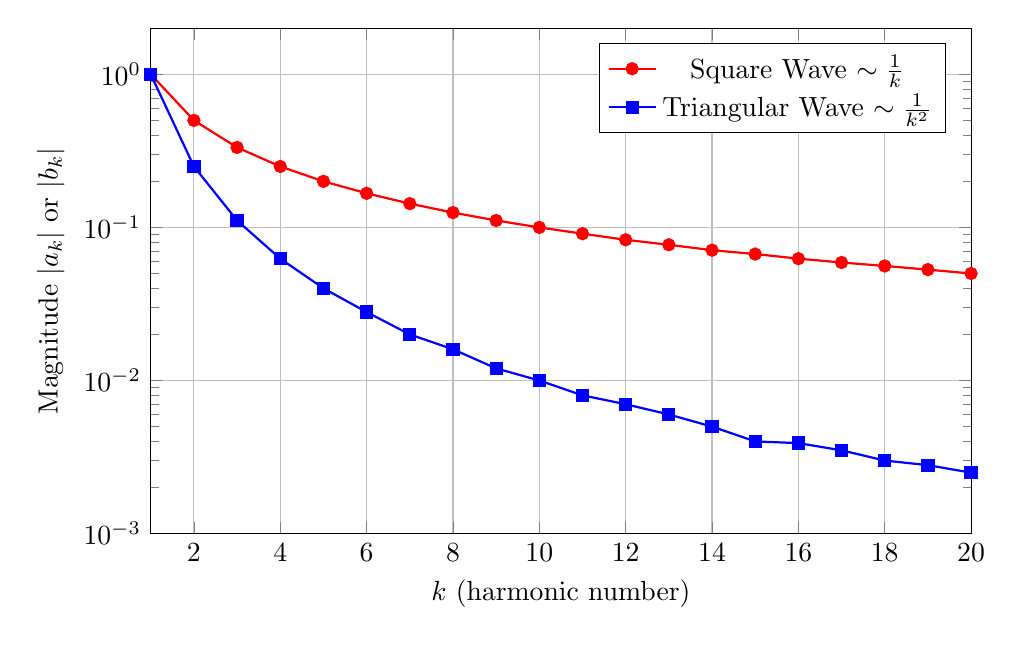
\begin{tikzpicture}
\begin{axis}[
    xlabel={$k$ (harmonic number)},
    ylabel={Magnitude $|a_k|$ or $|b_k|$},
    legend pos=north east,
    grid=major,
    ymode=log,
    xmin=1, xmax=20,
    ymin=0.001, ymax=2,
    width=12cm,
    height=8cm
]
% Square wave: 1/k decay
\addplot[red, thick, mark=*, mark size=2pt] coordinates {
    (1,1) (2,0.5) (3,0.333) (4,0.25) (5,0.2) 
    (6,0.167) (7,0.143) (8,0.125) (9,0.111) (10,0.1)
    (11,0.091) (12,0.083) (13,0.077) (14,0.071) (15,0.067)
    (16,0.0625) (17,0.059) (18,0.056) (19,0.053) (20,0.05)
};
\addlegendentry{Square Wave $\sim \frac{1}{k}$}
% Triangular wave: 1/k^2 decay
\addplot[blue, thick, mark=square*, mark size=2pt] coordinates {
    (1,1) (2,0.25) (3,0.111) (4,0.0625) (5,0.04) 
    (6,0.028) (7,0.02) (8,0.016) (9,0.012) (10,0.01)
    (11,0.008) (12,0.007) (13,0.006) (14,0.005) (15,0.004)
    (16,0.0039) (17,0.0035) (18,0.003) (19,0.0028) (20,0.0025)
};
\addlegendentry{Triangular Wave $\sim \frac{1}{k^2}$}
\end{axis}
\end{tikzpicture}
